\section{Results}
\label{sec-results}
%\input graphsize_table
We will begin analysing the effectiveness of our new symmetry
reduction methods by comparing against results published in 
\cite{harabor10}. 
Next, we compare and contrast the performance of RSR with
the Swamps algorithm described in \cite{pochter10}.
Finally, we demonstrate the relative strengths and weaknesses of these two
techniques by scaling all maps in our benchmark sets by a factor of 3 and looking
at the effect this has on performance.

\begin{figure*}[t]
       \begin{center}
                       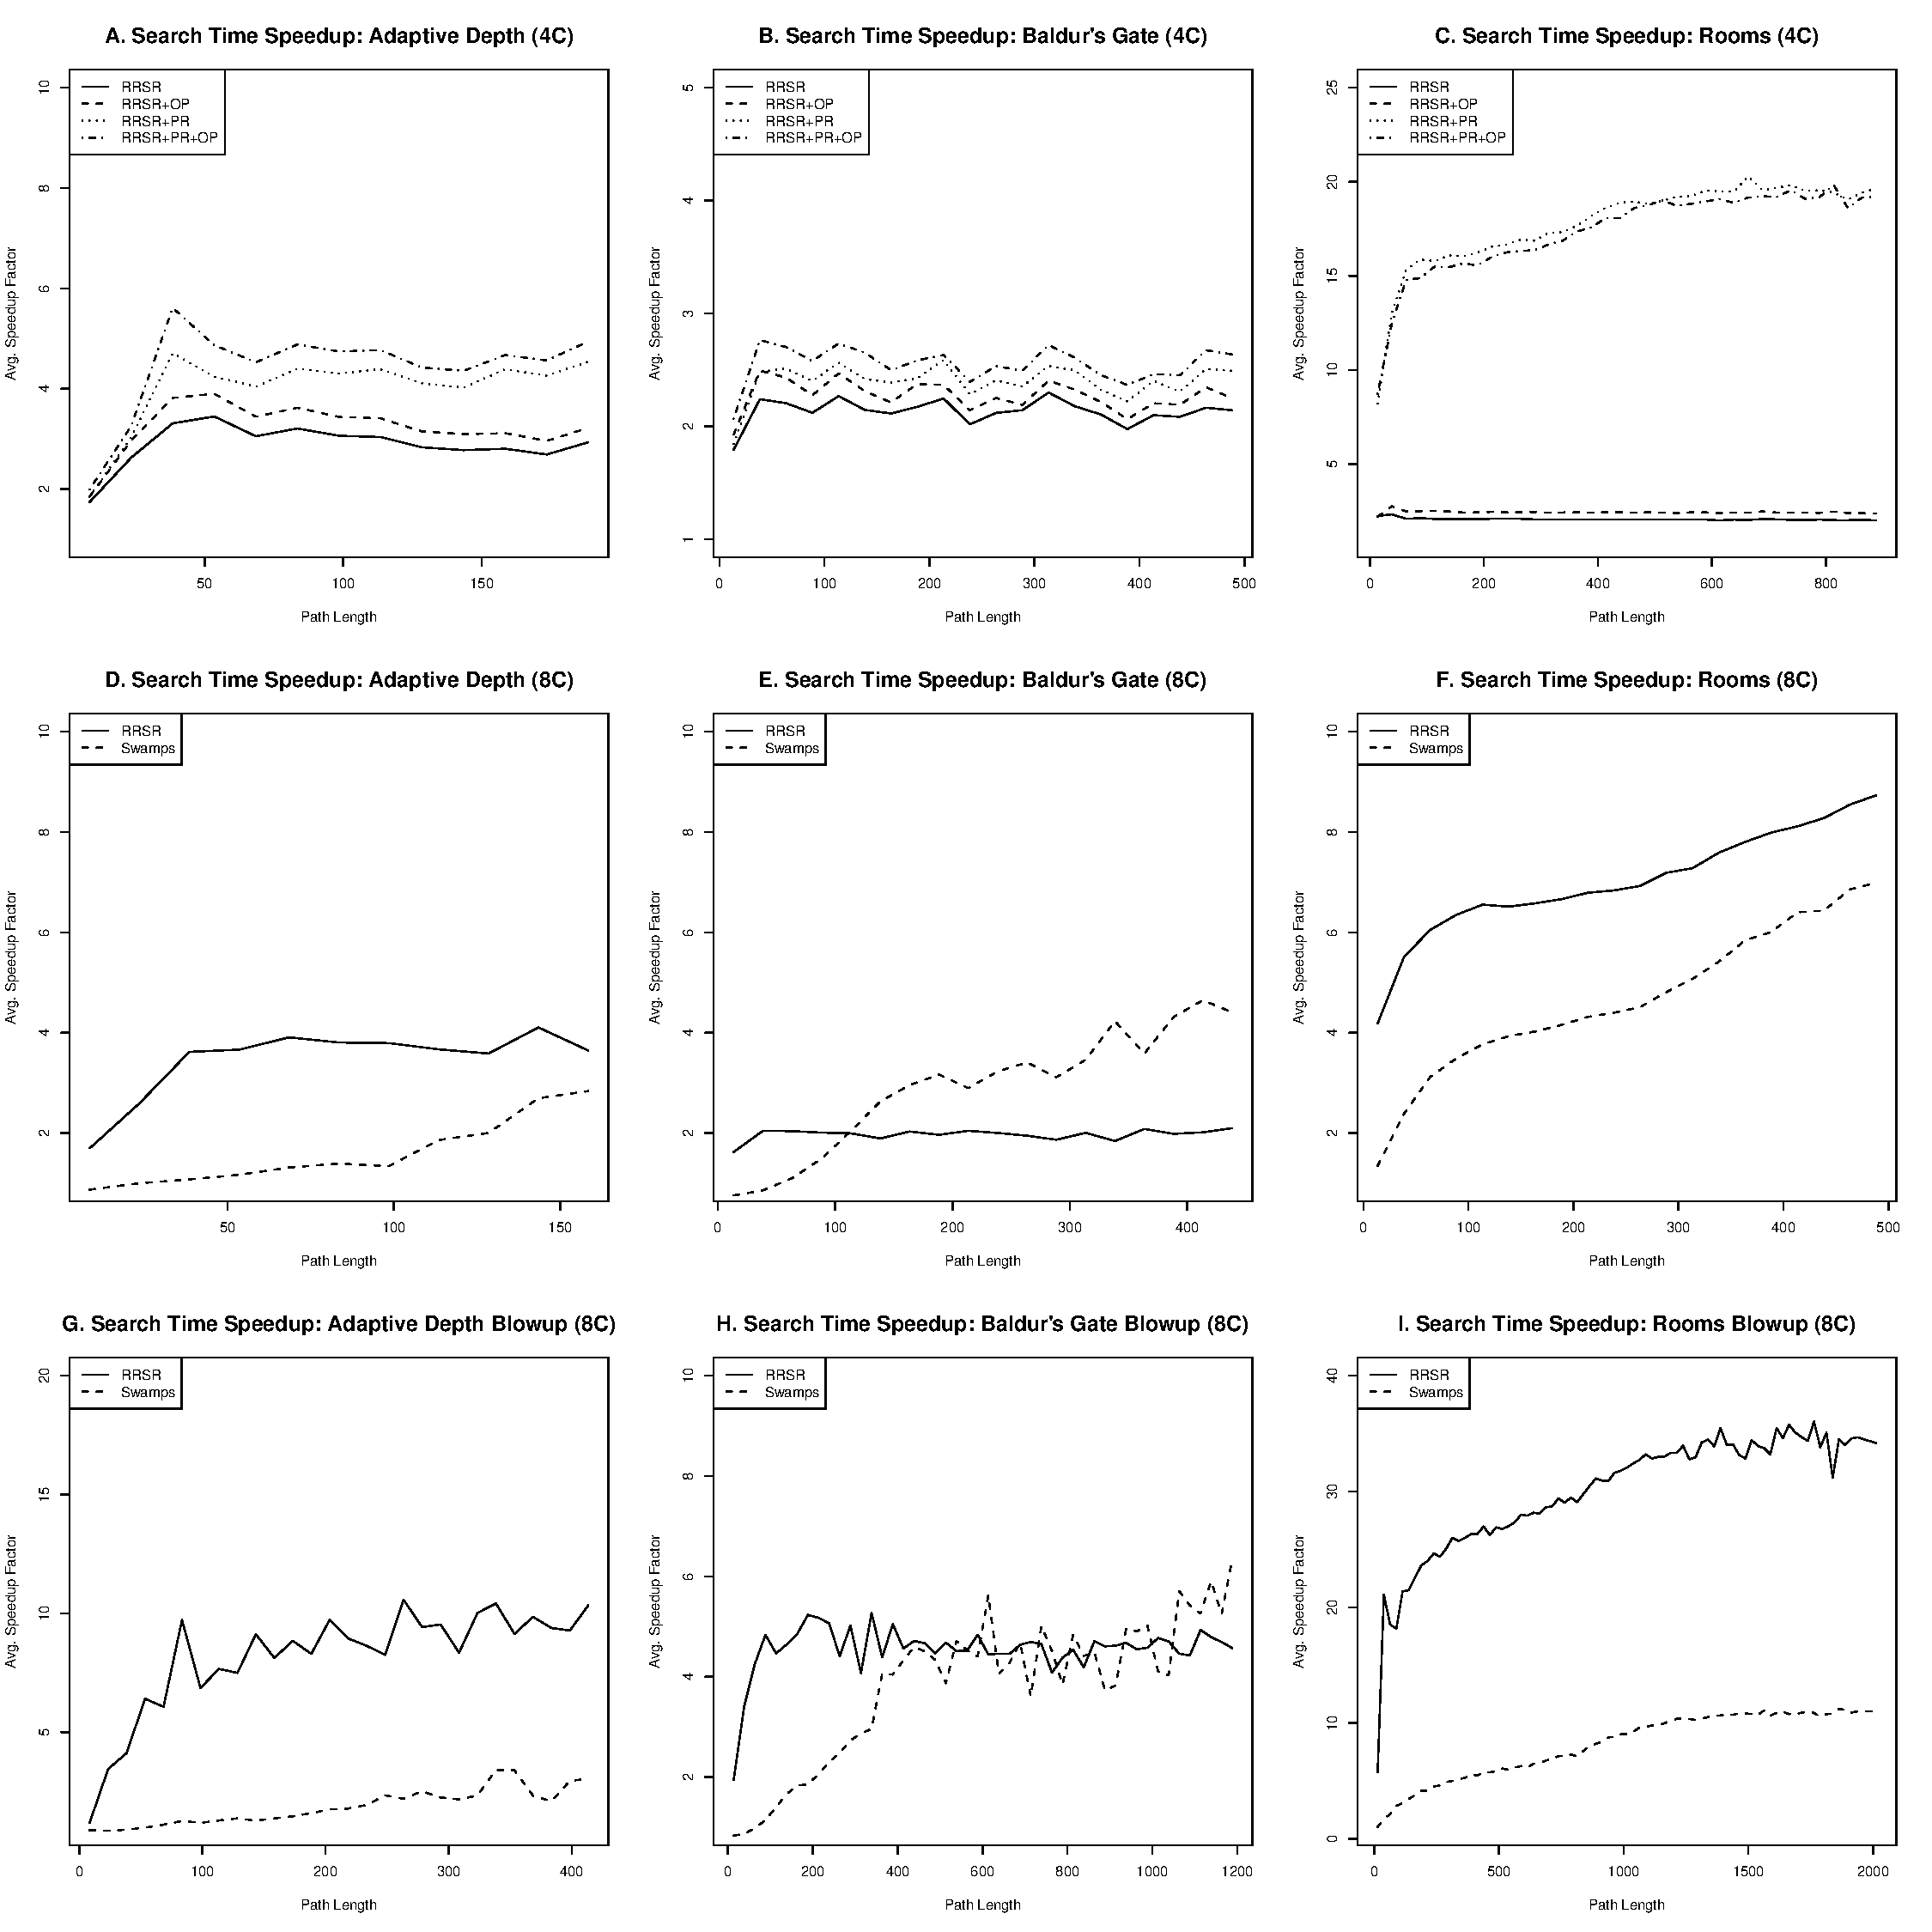
\includegraphics[width=1.95\columnwidth, trim = 10mm 10mm 10mm 0mm]{diagrams/speedup.pdf}
       \end{center}
       \caption{Average A* speedup on each of our three benchmarks. 
		Results are given in terms of search time.}
\label{fig-speedup}
\end{figure*}

We will discuss performance in terms of search time and measure
the average speedup experienced by A* when running on our modified 
grid maps as compared to the original. Using this metric
a speedup of 2.0 is twice as fast, 3.0 is three times as fast and so on
(higher is better).

\textbf{Comparison with 4ERR and Impact of PR and OP:}
In Figure \ref{fig-speedup} (A to C) we report on the 
effectiveness of offline perimeter reduction (PR) and online 
node pruning (OP) to speeding up A*.
The comparison includes not only our system
but also the 4ERR algorithm originally described by \citeauthor{harabor10}~\shortcite{harabor10}.
Furtheremore, to measure the individual impact of each of our speedup enhancements
we develop and include in the comparison two intermediate algorithms: 4ERR+OP and 4ERR+PR.
Here we restrict our attention to 4-connected grid maps,
since 4ERR does not work on the 8-connected variant.
\par
Perhaps the first thing to note is that RSR shows a convincing 
speed-up improvement over 4ERR and all its variants across all input maps.
%In addition, our work broadens the applicability of empty room abstraction
%to 8-connected maps.
%These two features allow us to conclude that using our enhancements is a better
%choice than using 4ERR alone.
This allows us to conclude that that RSR is a better choice than 4ERR on
4-connected maps.
\par
When analysing the impact of each enhancement,
we note that the single biggest improvement on each
benchmark is observed when applying perimeter reduction to the basic 4ERR method.
In the case of the Rooms benchmark (Figure \ref{fig-speedup}C) 4ERR+PR is over
18 times faster than A* search on an unmodified grid map.
Meanwhile, 4ERR alone only manages a 2 times speedup.
Smaller but still significant gains are also observed on the remaining two benchmarks:
on Adaptive Depth (Figure \ref{fig-speedup}A) 4ERR+PR is twice as fast as 4ERR alone
and on Baldur's Gate (Figure \ref{fig-speedup}B) 4ERR+PR improves on
the performance of 4ERR by over 10\%.
By comparison, 4ERR+OP yields much smaller gains across the same
benchmarks: usually beating 4ERR by between 10-12\%
In an additional experiment, we evaluated the impact of OP on 8-connected
grids and observed that its contribution to speedup was more significant than in 
the 4-connected case.
This can be explained as follows: on 4-connected maps, 4ERR maintains a very low
branching factor, which is comparable (and even slightly better) than the branching
factor on the original map. 
On the other hand, 8ERR (i.e. RSR without OP and PR speedup enhancements) 
can introduce larger branching factors. Therefore, there are more opportunities for 
online pruning in the latter case. 
Other details (and charts) are left out because of room limitations.
\par
Finally, it is interesting to note the sometimes large performance variation 
from one benchmark to another. This is indicative of how effectively we can 
decompose the different maps into rectangular shaped regions.
For example, the maps in the Rooms set are highly suited to this approach but those
from Baldur's Gate, which have an unusual 45-degree orientation, are not.
In such cases there are fewer opportunities to build large empty rooms and to apply perimeter reduction.
This leads to larger search spaces and reduced performance. 
\par
\textbf{Comparison to Swamps:}
Next, we compare the speedup performance of RSR with the swamps algorithm
of \citeauthor{pochter10}~\shortcite{pochter10}.
To undertake our evaluation, we used the authors' source code and ran all experiments 
using their recommended running parameters:
%\footnote{To the best of our knowledge 
%these parameters are unpublished; they were recommended to us in a private
%communication.}:
a swamp seed radius of 6 and ``no change limit'' of 2.
\par
Figure \ref{fig-speedup} (D to F) gives search time speedup results for both 
RSR and swamps running on the 8-connected variants of our three benchmark 
problem sets. 
On Adaptive Depth (Figure \ref{fig-speedup}D), we observe that 
swamps yields a maximum search time speedup of 2.8 times faster than 
 A* running on an unmodified grid map; however this is only true for problems of length greater than 150.
By comparison RSR yields a maximum speedup of 4.1 with comparatively little fluctuation across the
large majority of problem instances.
On Baldur's Gate (Figure \ref{fig-speedup}E) this trend is almost reversed; RSR consistently 
yields search time speedups of factor 2 while swamps exhibits a maximum speedup of 4.4.
Finally, on Rooms (Figure \ref{fig-speedup}F) RSR is again shown to be faster than swamps;
usually by a factor of between 2 and 3 across most problem instances.
\par
In the benchmarks which RSR does best (Rooms, Adaptive Depth) 
there are usually large open areas and the terrain can often be naturally decomposed into rectangular rooms.
At the same time, swamps-based reduction appears to be much better suited for identifying symmetric paths 
in graphs where this is not the case.
\par
\textbf{Effect of Obstacle Density:}
To better understand the effect that obstacle density has on the search performance of the two algorithms
we scaled up each map in every benchmark by a factor of 3 and generated a new
set of 100 random problem instances per map.
Scaling each of the benchmarks in this way has the effect of producing larger open areas and allows 
us to measure the impact of this variable on search time speedup.
In the following analysis we will contrast the new
results with the observed speedup for problems of the same length on the un-scaled maps.
\par
Figure \ref{fig-speedup} (G to I) gives search time speedup performance for both RSR and swamps
on each of the scaled-up benchmarks.
On Adaptive Depth (Figure \ref{fig-speedup}G), the average search time speedup of RSR reaches a maximum of 10. 
By comparison, swamps reaches a maximum speedup factor of 3.
When we limit our attention to problem instances of length less than 170 we observe that the speedup 
for RSR has increased, from 4 to 9, when compared to its performance for similar-length problems on the original 
unscaled maps (Figure \ref{fig-speedup}D). 
At the same time, the performance of swamps has decreased: from 2.8 to 1.2.
Turning our attention to Baldur's Gate (Figure \ref{fig-speedup}H) we observe a similar trend.
Although swamps has a higher maximum speedup than RSR (6.4 vs. 5.3), the performance of the two 
algorithms is very similar across a wide range of problem instances (450-1000).
RSR is clearly faster on instances whose path length is less than 400.
When we limit our attention to problem of length less than 450 we observe that the speedup experienced by
RSR has increased, from 2 to 4.5, when compared to its performance on the original unscaled maps
(Figure \ref{fig-speedup}E).
Meanwhile, the performance of swamps has decreased and is now dominated by RSR.
Finally we turn our attention to the scaled-up Rooms benchmark (Figure \ref{fig-speedup}I).
Here, the increase in size and naturally rectangular topography of the maps in this benchmark
has had a dramatic effect on RSR speedup, increasing it to over 30 for many
instances and reaching a maximum of 36 times speedup.
swamps also exhibits up to a 10 times speedup but if we limit our attention to problems of
length less than 500 we again see a reduction in performance when compared to swamps speedup
on the original unscaled maps (Figure \ref{fig-speedup}F). 
\par
The observed performance characteristics of both swamps and RSR
are not unexpected.
The complementary tendencies of the two algorithms
are consistent with the fact that 
the basic ideas behind swamps and Empty Rectangular Rooms are quite different:
%By definition, a swamp requires that any two nodes adjacent to the swamp
%can be connected through an optimal path that does not intersect with the swamp.
%In contrast, in the case of empty rectangular rooms, 
%crossing the room is the only way to connect optimally nodes on (distinct edges of) the perimeter.
swamps prune out areas that can be avoided without introducing a detour while 
rectangle-based symmetry reduction allows for a faster exploration of areas that need to be searched.
%\par
%In the case of RSR we would expect performance to improve as the average size of
%rectangular rooms increases.
%Larger rooms allow us to prune a larger number of interior tiles and we would expect this to be reflected
%by an associated increase in speedup. This was indeed the case in our measurements.
%In the case of swamps, we would expect the opposite to occur. As the average size of each swamp increases
%there are more tiles to be considered per search. Since the algorithm does not attempt to speed up searching
%\emph{inside} a swamp, each swamp traversal takes longer and we would expect to see this reflected
%by an associated decrease in speedup. As before, this was indeed the case.
%\par
Since it appears that the two algorithms are orthogonal, a natural extension of this work would 
be to create a new symmetry-based search space reduction which combines the two: 
first, apply 4(or 8)ERR+PR (as appropriate) to a grid in order to eliminate as many interior tiles 
as possible; then, apply a swamps-based decomposition to the resultant graph.
